\chapter{Dynamic reorganization of neuronal activity patterns in parietal cortex} 

\vspace*{-44pt}

Laura N. Driscoll, Noah L. Pettit, Selmaan N. Chettih, Matthias Minderer, and Christopher D. Harvey

\smallskip
\textit{This and the following chapters are a modified version of a submitted manuscript.}

\vspace*{50pt}

\section{Introduction} \label{sec:chap3_intro}


Here we monitored cortical representations of learned associations between arbitrary stimulus-action pairings after these associations had been learned to expert levels. We developed methods to track the activity of populations of neurons and behavioral patterns across weeks as mice performed a navigation-based decision task in virtual reality at near-perfect levels. We focused on activity in the posterior parietal cortex (PPC), which is essential for performing the task and in rodents is considered to function in learned sensorimotor associations, including during navigation \citep{Harvey:2012du, McNaughton1994, Nitz2006, Whitlock2012}. We found that activity patterns changed greatly over the course of days and weeks, such that the population of neurons that provided the most task-relevant information drifted over time. Despite single cell changes over time, the PPC population maintained a steady state with the same statistics of population activity across weeks, such as, for example, a consistent distribution of the fraction of neurons active at each point in the trial. Information about the task could be decoded stably across time using a readout of population activity despite changes in individual neurons, and representations of newly learned cue-response relationships could be incorporated without perturbing existing representations. Our results reveal that single cell representations for learned associations are not stable across long time periods; rather, stability in neuronal representations is maintained at the population level. We propose that drift in neuronal activity patterns could be important for mediating a tradeoff between stable encoding of information and flexibility for incorporating new information.

\section{Results} \label{sec:chap3_results}

We trained mice to perform a navigation based two-alternative forced-choice task. Mice navigated through a T-maze in visual virtual reality  \citep{Harvey:2012du} (Figure \ref{fig:1_w_out_inact} a). Mice saw one of two possible visual cues (white walls or black walls) throughout the first half of the T-stem. Mice then ran through a delay period in the second half of the T-stem in which the walls were identical between trial types. At the T-intersection, mice had to report a choice about the cue identity by making a left or right turn for a condensed milk reward. Mice learned this task over 4-6 weeks of training and reached expert behavioral performance that was mostly stable over weeks (Figure \ref{fig:1_w_out_inact} b). 

\begin{figure}
\includegraphics[width=\textwidth]{figures/1_w_out_inact.pdf}
\caption[Chronic imaging during stable performance of a virtual-navigation decision task.]{\textbf{Chronic imaging during stable performance of a virtual-navigation decision task. a,} Schematic of the two trial types based on a virtual T-maze. Patterns indicate those presented on the virtual maze walls.
%
\textbf{b,} Behavioral performance on individual imaging days for each mouse. 
%
\textbf{c,} Example images of GCaMP6m-expressing neurons across days. One of four imaging planes from volumetric imaging is shown. Some examples of cells identified across days are colored. 
%
\textbf{d,} The activity of three example cells over three weeks. Left columns: mean GCaMP6m fluorescence image. Middle columns: deconvolved fluorescence signal on individual correct white cue-left turn and black cue-right turn trials. Right columns: mean activity on correct white cue-left turn (blue) and black cue-right turn (red) trials. See Methods \ref{fig:cell_selection} for cell identification protocol across days. 
\label{fig:1_w_out_inact}}
\end{figure}

\subsection{Tracking behavior and neuronal activity over weeks} \label{sec:chap3_track_neuron_behavior}

During the task, we imaged the activity of hundreds of layer 2/3 PPC neurons simultaneously using volumetric two-photon calcium imaging. Imaging locations were identified based on stereotaxic coordinates, and separate experiments revealed that these coordinates corresponded to a location anterior to cortical regions identified using retinotopic mapping (Figure \ref{fig:widefield}). Here we call this region PPC and note that recent work from the Allen Brain Institute calls this region VisA  \citep{CCF2015} and that this region is medial to what previous work has called secondary visual area A \citep{Wang2007} (Methods \ref{methods:ppc}). Imaging sessions were performed typically every day with occasional one-day gaps between sessions (Figure \ref{fig:cell_selection}). On each day we identified the same field-of-view so that we could track activity patterns of neurons across time (Figure \ref{fig:1_w_out_inact} c-d). We developed a conservative approach to ensure as best as possible that we identified the same neurons across imaging days. First, we identified fluorescence signal sources (putative cells) on each day independently. Signal sources were selected on the basis of temporally correlated fluctuations between pixels, rather than using manual, anatomical selection methods that can fail to separate nearby cells, dendrites, and axons \citep{Hamel2015, Peron2015}. Second, to match putative cells across all imaging days, we used a custom algorithm based on distance between regions-of-interest (ROIs) and similarities in the fluorescence images surrounding each ROI. Finally, we visually compared each identified cell across all days to ensure that each cell appeared consistent in the anatomical images and had highly similar ROIs assigned to it (Figure \ref{fig:cell_selection}). We only considered cells on days in which they were identified; other days, in which we could not with high confidence identify the cell, were excluded from our analysis, such that not every cell was identified on every day. This approach was aimed to minimize mislabeling of neurons across days and was intended to be conservative compared to previously developed methods \citep{Huber2012, Liberti2016, Peron2015, Peters2014, Poort2015, Ziv2013} (see Figure \ref{fig:cell_selection} and Methods \ref{methods:across days} for a full discussion).  

\subsection{Necessity of PPC activity for post-learning performance of the task} \label{sec:chap3_necessity}

The activity patterns of PPC neurons on a single imaging day were consistent with those reported previously \citep{Harvey:2012du, Morcos2016}. On each day, individual neurons were transiently active, with different neurons active at different time points, such that PPC activity tiled the entire duration of a trial (Figure \ref{fig:1_seq_inact} a). Many of these responses were reliable and selective for a particular trial type. For example, some cells were more active on black cue-right turn trials than on white cue-left turn trials or vice versa.

\begin{figure}
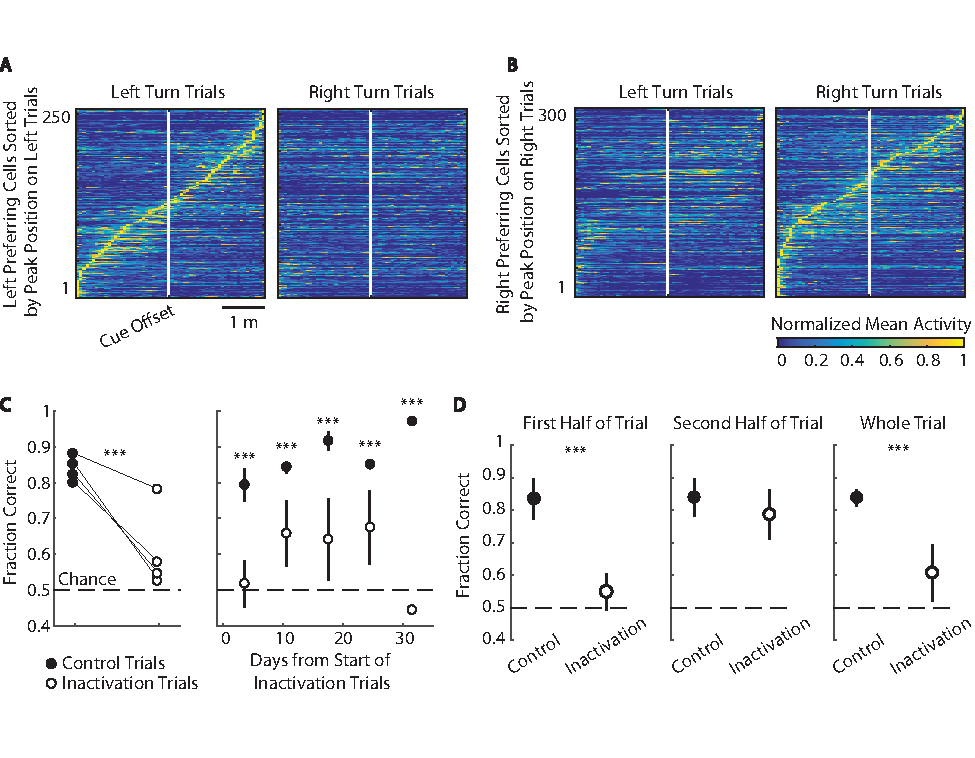
\includegraphics[width=\textwidth]{figures/1_seq_inact.pdf}
\caption[Neuronal population dynamics and inactivation experiments.]{\textbf{Neuronal population dynamics and inactivation experiments. a-b,} Mean activity of neurons with a significant peak of activity on \textbf{a} left turn trials and \textbf{b} right turn trials (Methods \ref{methods:peaks}) from 5 mice. Traces were normalized to the peak of each cell's mean activity on preferred trials from a single day and sorted by the peak position. 
%
\textbf{c,} Left: Task performance on optogenetic PPC inactivation and control trials for 4 mice. Trials were combined across multiple days. No significant effect was observed for a control mouse not expressing ChR2: p = 0.18. Right: Task performance for inactivation and control trials within non-overlapping 7 day time bins. Error bars indicate mean $\pm$ sem for n=3,3,4,2,1 mice for each of the time bins, respectively. $***$ indicates p < 0.001 between control and inactivation trials (bootstrap analysis with shuffled trial labels).
%
\textbf{d,} Optogenetic inactivation during the first half of the T-stem (left), second half of the T-stem (middle), and entire T-stem (right). For each manipulation, trials were pooled across multiple sessions. Points indicate mean $\pm$ sem. n=4 mice. $***$ indicates p < 0.001 based on bootstrap shuffle of control and inactivation trial labels. p = 0.06 for the second half of the T-stem (middle).
\label{fig:1_seq_inact}}
\end{figure}

\bigskip

The activity in the PPC appeared necessary for the mouse to perform the behavioral task. We virally expressed channelrhodopsin-2 in parvalbumin-expressing inhibitory interneurons at a location centered at the PPC and activated these neurons to inhibit excitatory activity on a subset of trials. Inactivation of PPC decreased the behavioral performance of the mouse from ~85 $\%$  correct to just above chance levels (Figure \ref{fig:1_seq_inact} c). These results were obtained days or weeks after the mouse achieved plateau behavioral performance, suggesting that PPC activity was necessary for performing the task even in the post-learning phase. These results were in agreement with earlier work that used pharmacological methods to inactivate the PPC and other studies showing a role for the rodent PPC in visual decision tasks \citep{Goard2016, Harvey:2012du, Licata2016, Raposo2014}. To futher resolve the role of PPC in this task, we then inhibited PPC activity at different segments, either during the first half of the trial or the second half of the trial. Interestingly, we found that when PPC activity was inhibited in the first half of the trial, the mouse's performance was greatly impaired (Figure \ref{fig:1_seq_inact} d). In contrast, inhibiting PPC activity during the second half the trial had no significant effect (p = 0.06) on the mouse's performance (Figure \ref{fig:1_seq_inact} d). This result is consistent with what has been reported previously in other tasks \citep{Goard2016, Licata2016, Raposo2014}. We note that it is difficult to interpret what this finding means in terms of PPC's role in the task: PPC activity could be involved in the transformation of the sensory information into a behavioral action plan or in some aspect of visual processing or potentially other computations. We also note that although inactivation was centered on PPC, such activity manipulations may not be isolated solely to PPC, as has been shown in other systems \citep{Otchy2015}.

\subsection{Reorganization of sequential activity across maze locations} \label{sec:chap3_peaks}
To compare the activity patterns of neurons across days, we first focused on sequential activity throughout a trial. On each day, a sequence of neuronal activity was present (Figure \ref{fig:2_all} a), top left, center, and bottom right panels). To determine whether this sequence of activity was the same from day to day, we sorted neurons based on where in the maze they had a reliable peak of activity. We then used the same sorting to look for the same sequence of activity on earlier or later days. Strikingly, the sequence of activity that was present on one day was largely different on other days (Figure \ref{fig:2_all} a). Cells that had a significant peak of activity in the maze on a given day were unlikely to have a significant peak of activity at the same or nearby position after long intervals (Figure \ref{fig:2_all} b). Over time this likelihood of a consistent peak position approached levels expected from a random reorganization of neuronal identities (Figure \ref{fig:2_all} b). These changes resulted from cells with a peak of activity on one day either losing that peak of activity or having a shift in the peak location on subsequent days, both of which increased in likelihood as a function of time from when a peak was identified (Figure \ref{fig:2_all} d). In some cases, peaks shifted by distances larger than one meter. The loss of peaks of activity was offset by an approximately constant rate at which cells initially lacking a peak of activity gained an activity peak (Figure \ref{fig:2_all} d), resulting in a consistent fraction of active cells with significant peaks over the imaging period of weeks (22.0 $\pm$ 0.5$\%$ of neurons, mean $\pm$ sem) (Figure \ref{fig:2_all} c). Together these results indicate that the same activity patterns were not repeated for long time periods.

\begin{figure}
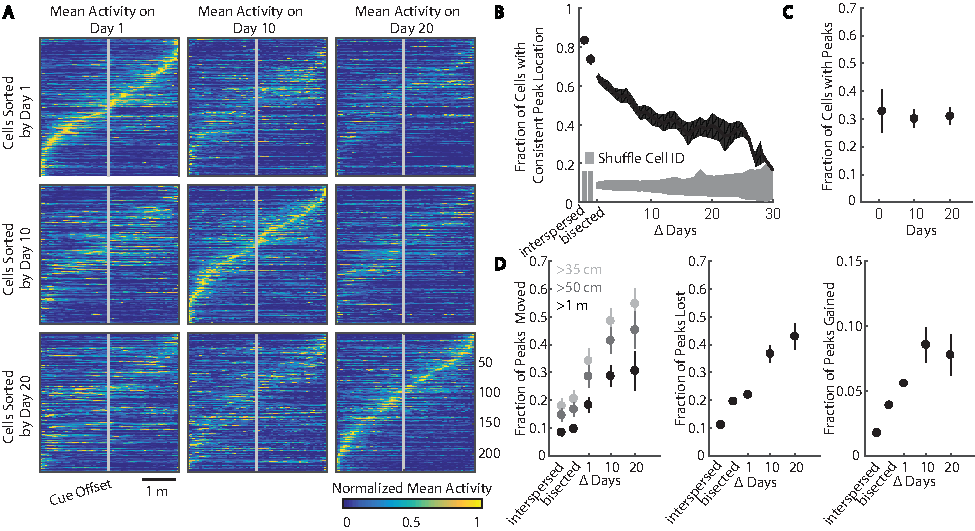
\includegraphics[width=\textwidth]{figures/2_all.pdf}
\caption[Reorganization of activity within a trial across days.]{\textbf{Reorganization of activity within a trial across days. a,} Normalized mean activity of neurons that were identified on all three imaging days (1, 10 and 20) and that had a statistically significant peak in the sorted day (95 $\%$ confidence). Sorting was the same for each day within a row and was different across rows. Gray lines indicate cue offset.
%
\textbf{b,} For all cells with a highly significant (99 $\%$ confidence) peak of activity on a given day, the fraction of cells that had a significant(95 $\%$ confidence) peak of activity at a similar location (< 70 cm shift) on a subsequent day. Shading indicates mean $\pm$ sem (n = 5 mice; some large interval data points had fewer than 5 mice, see Figure \ref{fig:cell_selection}. The gray shaded area indicates 95 $\%$ confidence intervals of chance levels based on shuffling the cell IDs separately on each day. Fraction of cells with consistent peak location vs. time: p < $10^{-8}$, ANOVA. Interspersed and bisected groups correspond to comparisons across half of data within a given session that was either interspersed throughout the session, or divided into first and second halves.
%
\textbf{c,} Fraction of cells that had a significant peak on the noted day.  Fraction vs. time: p =  0.85, ANOVA. In panels \textbf{c-d}, error bars indicate mean $\pm$ sem, n = 5,5,4 mice for the time intervals shown.
%
\textbf{d,} Left: For cells with a significant peak on day n and day n+x, the fraction of peaks that shifted by greater than 35 cm, 50 cm and 1 m. Fraction moved 35 cm vs. time: p = 0.019, ANOVA. Center: For cells with a highly significant peak on day n, the fraction of cells that did not have a significant peak on day n+x. Fraction lost vs. time: p < $10^{-9}$, ANOVA. Right: For cells without a significant peak of activity on day n, the fraction of cells that had a highly significant peak on day n+x.  Fraction gained vs. time: p = 0.96 ANOVA.  Interspersed and bisected groups correspond to comparisons across half of data within a given session that was either interspersed throughout the session, or divided into first and second halves.
\label{fig:2_all}}
\end{figure}

\subsection{Different populations of neurons with trial type-specific activity patterns across days} \label{sec:chap3_single_cell_decoding}
We also investigated changes in activity patterns that could be related to information about the trial type. Specifically, we asked if the neurons that had different activity patterns on trials with different cues and choices, and thus provided information potentially useful for solving the task, were the same across time. For each neuron on each day, we used a decoder to quantify how well that neuron's activity across the entire duration of a single trial could predict the trial type (white cue-left turn vs. black cue-right turn, correct trials only). On a given day, a significant fraction of active neurons had a decoding accuracy above chance (29.1 $\pm$ 1.1$\%$ of neurons, mean $\pm$ sem, with p < 0.05 compared to decoding with shuffled trial labels). Neurons that had high decoding accuracies on a given day, and thus different activity patterns between trial types, did not necessarily have significant decoding accuracies on subsequent days (Figure \ref{fig:3_all} a-b). The large majority of neurons that were identified on more than 15 imaging days only had above chance decoding accuracy on less than half of those days (Figure \ref{fig:3_all} c). Moreover, only 1.6$\%$ of these neurons had significant decoding accuracy on all days in which they were identified. The likelihood that a cell with greater than chance decoding accuracy on a given day also had significant decoding accuracy on a subsequent day decreased with the interval between compared days (Figure \ref{fig:3_all} d). Over time the likelihood that a cell maintained significant decoding accuracy decreased to levels approaching those consistent with a random reorganization of cell identities (Figure \ref{fig:3_all} d). We tracked the subpopulation of neurons that was the most highly informative about trial type on a given day. Over time, the distribution of decoding accuracy within this subpopulation approached and largely overlapped with the distribution of the entire population, indicating that this subpopulation was not a special set of highly selective neurons across all time points (Figure \ref{fig:3_all} e).

\begin{figure}
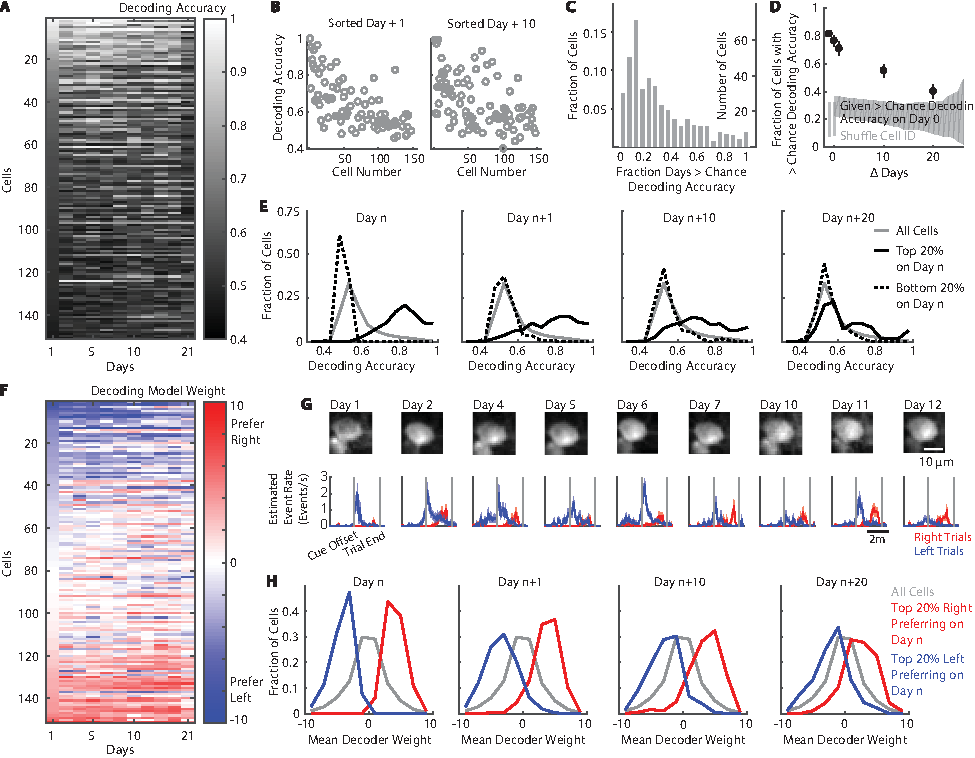
\includegraphics[width=\textwidth]{figures/3_all.pdf}
\caption[Reorganization of information about trial-type across days]{\textbf{Reorganization of information about trial-type across days a,} Decoding accuracy for trial type based on the activity of individual neurons, sorted by decoding accuracy on Day 1. 
%
\textbf{b,} For an example day, cells were sorted by their trial-type decoding accuracy. Decoding accuracy is shown for a held out set of data on the day used for sorting (black) and on subsequent days (gray). 
%
\textbf{c,} For the cells that were identified on $\ge$ 15 days, the fraction of days in which a cell's activity provided above chance decoding accuracy, relative to the number of days in which the cell was identified. Chance was determined as p < 0.05 (bootstrap analysis with shuffled trial labels). 
%
\textbf{d,} Given high confidence for significant decoding accuracy on day n (real data performed better than 990 of 1000 shuffles), the fraction of cells with greater than chance decoding accuracy (real data performed better than 950 of 1000 shuffles) on day n+x. Interspersed and half groups indicate fraction of cells with consistent decoding accuracy across odd/even trials and first/second half of trials respectively. Error bars indicate mean $\pm$ sem n = 5 mice. The gray shaded area indicates 95 $\%$ confidence intervals of chance levels based on shuffling the cell IDs separately on each day. Fraction of cells that maintain significant decoding accuracy vs. time: p < $10^{-11}$, ANOVA.
%
\textbf{e,}  On a given day, the cells with the top 20 $\%$ and bottom 20 $\%$ of decoding accuracies were identified. The distributions of decoding accuracy for these cells are shown in comparison to the distribution for all cells after intervals of 1, 10, and 20 days.
%
\textbf{f,} Trial type preference for the cells in panel A sorted by trial type preference on day 1. Model weights with positive values indicated higher activity on black cue-right turn trials. A model weight was determined at each spatial bin in the maze, and the mean weight was calculated for each cell. 
%
\textbf{g,} Example of a single cell with dynamic trial-type information. Top: mean fluorescence image of the cell body. Bottom: mean activity of the cell on correct white cue-left turn (blue) and black cue-right turn (red) trials. 
%
\textbf{h,} On a given day, the cells with the top 20 $\%$ largest weights for white cue-left turn and black cue-right turn trials were identified. The distributions of trial-type weights are shown in comparison to the distribution for all cells after intervals of 1, 10, and 20 days.
\label{fig:3_all}}
\end{figure}

\bigskip

We also examined if the neurons with selective activity for one trial type (e.g. black cue-right turn trials) switched to having a preference for the other trial type (e.g. white cue-left turn trials) (Figure \ref{fig:3_all} f-h). The most highly selective cells for each trial type over time often lost their selectivity or gained additional selectivity, at other points in the maze, for the other trial type (Figure \ref{fig:3_all} f-g). We tracked the neurons that had the strongest preferences for each trial type on a given day (Figure \ref{fig:3_all} h). Over days, the trial type preferences of these neurons approached that of the entire population. Only a small fraction of neurons switched from having statistically significantly higher activity on one trial type to having statistically significantly higher activity on the opposite trial type (4.7 $\pm$ 1.7$\%$ of cells, mean $\pm$ sem; lower bound for chance: 1.4 $\pm$ 0.7$\%$ based on switches within a day using a hold out set; upper bound for chance: 45 - 50$\%$ based on switches in selectivity when cell IDs were shuffled across days). Switches in trial type preferences were thus rare from one day to the next, and gains or losses of selectivity were more common. Together these results indicate that the population of neurons that had trial type-specific information was largely different across days, with larger differences in these populations over longer time windows. 

\subsection{Using a generalized linear model to compare relationships between neuronal activity and behavioral features across days} \label{sec:chap3_glm_intro}

These findings together provide evidence that major changes and reorganization of neuronal activity patterns occurred during stable performance of a behavioral task. However, these analyses only considered two aspects of the task (position in the maze and trial type) and did not include other task features that could potentially be represented in the neuronal activity. For example, PPC has been considered to be important for movement planning and could thus have activity related to the running patterns of the mouse \citep{Andersen2009, Nitz2006, Whitlock2012}. In addition, PPC receives inputs from visual areas and might have activity related to the movement of visual stimuli projected on the screen, such as during turning compared to forward motion \citep{Harvey:2012du, Oh2014}. We wanted to understand whether behavioral variability across days could explain the changes in neuronal activity or alternatively if these changes were due primarily to single neurons having different relationships between their activity and the behavior of the mouse across time. We therefore developed an approach to describe an individual neuron's activity on single days based on a large number of variables that described the task and mouse's behavior. We developed a generalized linear model (GLM) in which we modeled the activity of an individual neuron based on the running patterns of the mouse on the spherical treadmill, the virtual maze position (visual scene), the trial type, reward events, and whether the mouse was in the inter-trial interval period \citep{Friedman2010, Park2014} (Figure \ref{fig:4_glm_tutorial} and Figure \ref{fig:4_filters}). 

\begin{figure}
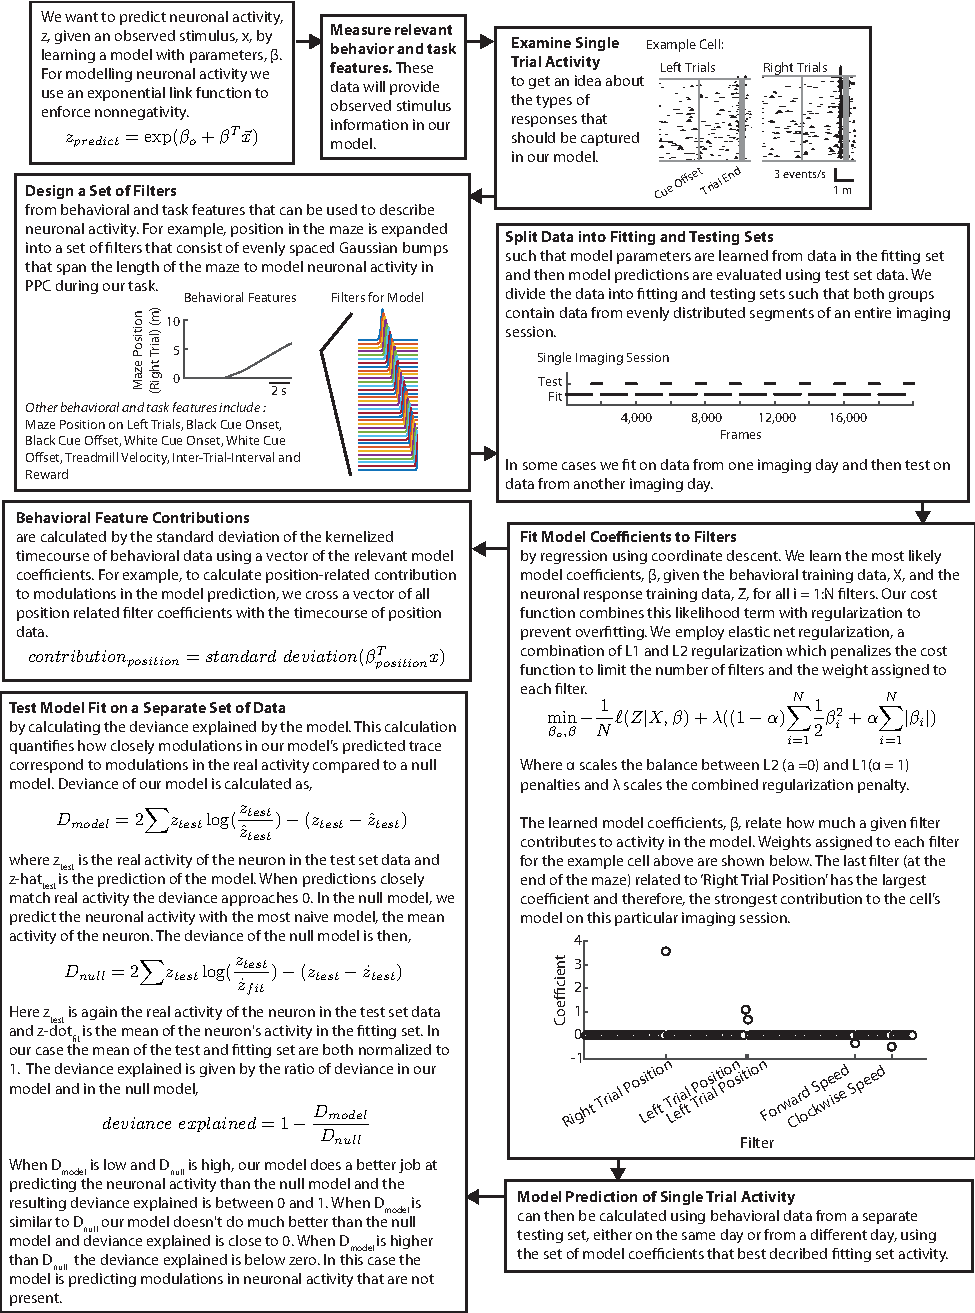
\includegraphics[width=\textwidth]{figures/4_glm_tutorial.pdf}
\caption[GLM fitting procedure]{\textbf{GLM fitting procedure}
\label{fig:4_glm_tutorial}}
\end{figure}

\begin{FPfigure}
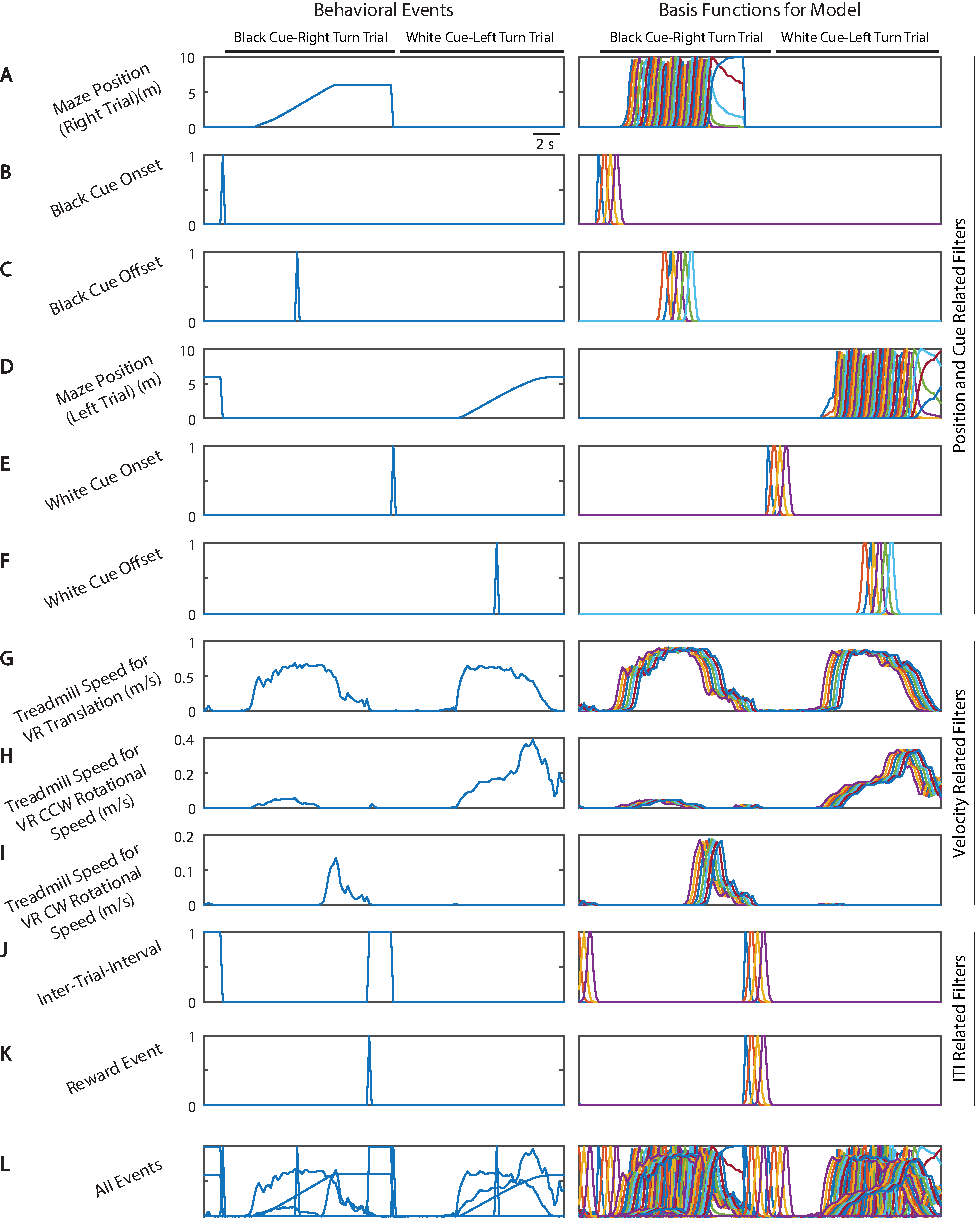
\includegraphics[width=\textwidth]{figures/4_filters.pdf}
\caption[Basis functions for encoding model.]{\textbf{Basis functions for encoding model.} Trial and behavioral measurements during each imaging frame (left) were expanded into a set of basis functions that were incorporated into the GLM (right). Filter groupings used in contribution calculation for Figure \ref{fig:6_decoding} shown in right margin.
\textbf{a,} Left: Maze position on right turn trials. Right: 36 spatial boxcar filters of position spanning the length of the maze were convolved with a Gaussian filter for right turn trials. 
%
\textbf{b,} Left: Black cue onset. Right: 4 Gaussian basis functions that span the first 2 seconds of black cue-right turn trials. 
%
\textbf{c,} Left: Black cue offset (delay period onset). Right: 6 total basis functions, 2 basis functions extended for 1 second preceding cue offset and 4 basis functions extended for 2 seconds following cue offset.
%
\textbf{d,} Left: Maze position on left turn trials. Right: 36 spatial boxcar filters of position spanning the length of the maze were convolved with a Gaussian filter for left turn trials.
%
\textbf{e,} Left: White cue onset. Right: 4 Gaussian basis functions that span the first 2 seconds of white cue-left turn trials. 
%
\textbf{f,} Left: White cue offset (delay period onset). Right: 6 total basis functions, 2 basis functions extended for 1 second preceding cue offset and 4 basis functions extended for 2 seconds following cue offset. 
%
\textbf{g-i,} Left: Movement of spherical treadmill. Right: 8 basis functions total for each of 3 running speed signals were extended 1 second forward and backward in time to model predictive and responsive signals.
%
\textbf{j,} Left: Inter-trial interval Right: 4 basis functions that extended for 2 seconds forward in time following trial end. 
%
\textbf{k,} Left: Inter-trial interval Right: 4 basis functions that extended for 2 seconds forward in time following reward.
%
\textbf{l,} Left: All trial and behavioral measurements. Right: All basis function for GLM, excluding novel cue onset and offset (same as black and white cue basis functions).
\label{fig:4_filters}}
\end{FPfigure}
%\afterpage{\clearpage}
\clearpage

\bigskip

We fit the relationship between a cell's activity and these behavior and task features to develop a model of that cell's activity-behavior relationship. We tested the quality of this model by predicting the cell's activity based on the behavioral and task features in a subset of trials not used for fitting. If the predicted activity closely matched the real activity, we concluded that our model could describe the activity-behavior relationship for the cell on that day. Across cells, models were able to explain a large fraction of neuronal activity (57.9 $\pm$ 2.6$\%$ of cells, mean $\pm$ sem, had significant fits measured as the explained deviance in the neuronal activity compared to a null model) (Figure \ref{fig:4_glm_fits} c). We fit separate models for each neuron on each day. The distribution of model prediction qualities for each day across the population was consistent throughout the duration of our several week study (Figure \ref{fig:4_glm_fits} d).

\begin{figure}
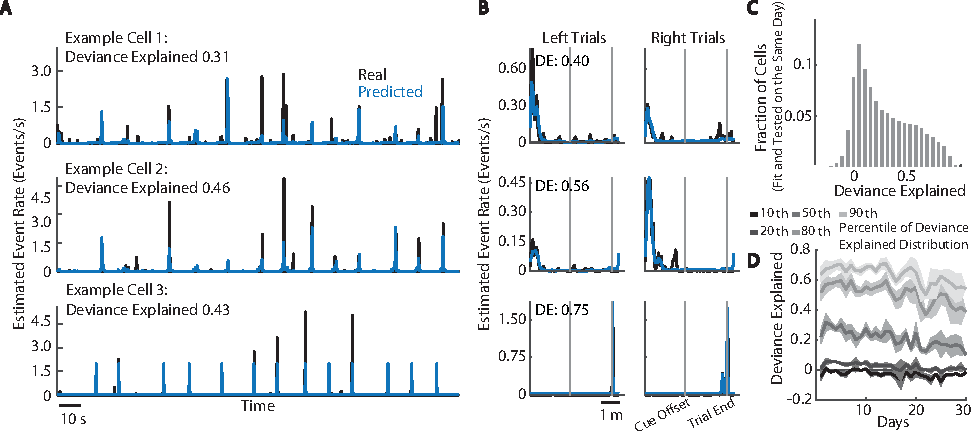
\includegraphics[width=\textwidth]{figures/4_glm_fits.pdf}
\caption[Fitting activity-behavior relationships with a generalized linear model.]{\textbf{Fitting activity-behavior relationships with a generalized linear model. a,} For three example cells, a segment of activity is shown (black) along with the activity predicted from the GLM (blue). Deviance explained is calculated directly from single frame predictions.
%
\textbf{b,} Same as in panel A, except for the mean activity on white cue-left turn and black cue-right turn trials. Deviance explained is calculated from trial averaged predictions, concatenated white cue-left turn and black cue-right turn mean activity.
%
\textbf{c,} Distribution of the quality of model fits measured by deviance explained compared to a null model for trial averaged predictions (Methods \ref{methods:analysis_of_model}). The model was fit and tested on data from the same day. n = 17,353 model fits across cells and days.
%
\textbf{d,} Distribution of deviance explained for models fit on each day divided into five groups. Similar distributions of fits were apparent on each day. Shaded regions indicate mean $\pm$ sem for n = 5 mice (fewer mice on some later days, see Figure \ref{fig:cell_selection} j for the number of mice at each interval).
\label{fig:4_glm_fits}}
\end{figure}

\bigskip

We used these models to compare the relationship between a cell's activity and behavioral features across days. Using the model of a cell's activity-behavior relationship fit on a single day, we predicted the cell's activity based on behavior features in other days (Figure \ref{fig:glm_across}). If the model developed on one day was able to predict activity on a subsequent day, then we concluded that a consistent activity-behavior relationship existed. In contrast, if a model developed on one day failed to predict the activity on subsequent days, then we concluded that a consistent activity-behavior relationship was absent. This approach has the potential to track stable relationships between neuronal activity and behavior features across days that traditional approaches might miss. For example, if a neuron had activity related to the running patterns of a mouse and if these running patterns changed relative to position in the maze across days, the GLM could potentially reveal a stable activity-behavior relationship over time that would be missed if only maze position were analyzed. Importantly, behavioral features, such as running speed and trial duration, were variable across trials, but maintained a similar distribution and range of values on each day, suggesting that models should be transferable across days (Figure \ref{fig:4_distribution_filters}). We limited effects due to fitting procedures, such as regularization, and due to correlated task variables by fitting and testing bidirectionally for each pair of days (see Methods \ref{methods:analysis_of_model} for a full discussion). 

\begin{figure}
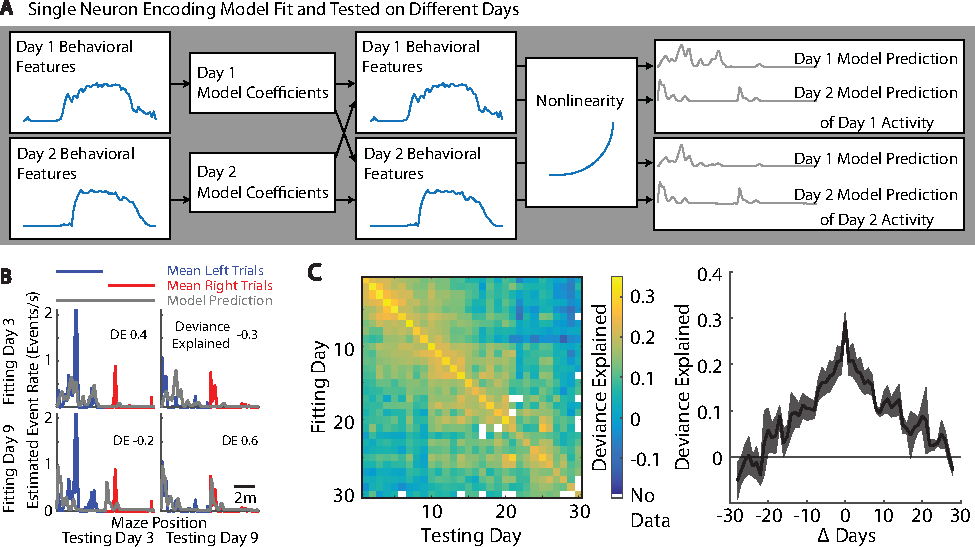
\includegraphics[width=\textwidth]{figures/4_glm_across_design.pdf}
\caption[Fitting activity-behavior relationships with a generalized linear model.]{\textbf{Fitting activity-behavior relationships with a generalized linear model. a,} For each neuron on each day, a separate generalized linear model was fit to the activity of the neuron based on behavior and task features. Each day's model was then tested for how well it could predict activity-behavior relationships on other days. Model coefficients for behavioral filters were fit on one day and then applied to behavioral data from another day to produce a prediction of the neuronal activity time course for that day.
%
\textbf{b,} For an example cell, mean activity for white cue-left turn (blue) and black cue-right turn (red) trials on imaging days 3 and 9. One model was fitted on data from day 3 and another model was fitted on data from day 9. Each model was used to make a prediction (gray) about the neuron's activity based on behavioral data in a test set, either from the same day or the other day. The model fit quality was quantified as the deviance explained. 
%
\textbf{c,} Left: Deviance explained by models fit on a one day and tested on the same or a different day. Values were averaged across all cells for each mouse and then averaged across mice. Each entry has a variable number of data points (and in some case no data points, white values) due to varying durations of imaging periods for mice and gaps between imaging days (Figure \ref{fig:cell_selection} k). Right: Average deviance explained as a function of time between the fitting and testing days. Shading indicates mean $\pm$ sem.
\label{fig:glm_across}}
\end{figure}

\begin{figure}
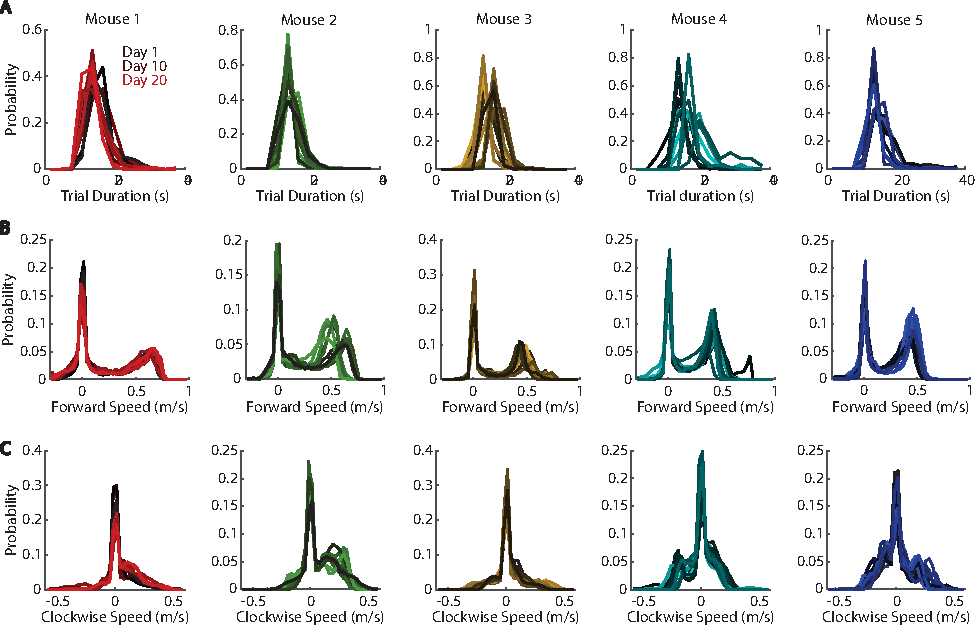
\includegraphics[width=\textwidth]{figures/4_distribution_filters.pdf}
\caption[Behavioral features were variable but had overlapping distributions across days]{\textbf{Behavioral features were variable but had overlapping distributions across days a,} For each mouse, the distribution of trial durations from cue onset to trial end. 
%
\textbf{b,} For each mouse, the distribution of treadmill speed for forward translation in the virtual environment (about the pitch axis relative to the mouse's body axis). 
%
\textbf{c,} For each mouse, the distribution of treadmill speed for rotation in the virtual environment (about the roll axis relative to the mouse's body).
\label{fig:4_distribution_filters}}
\end{figure}

\subsection{Changing activity-behavior relationships in single neurons over days} \label{sec:chap3_activity_behave_relation}

Models of activity-behavior relationships developed on a given day were, on average, able to predict activity patterns well on neighboring days, but did a poor job of predicting activity patterns as the time between the compared days increased (Figure \ref{fig:glm_across} c). Over long intervals, model predictions eventually reached that of a null model (for intervals greater than 17 days), indicating that a cell's activity-behavior relationship was generally inconsistent over weeks (Figure \ref{fig:glm_across} c). We also quantified similarity of models for a given cell across days using Kendall rank correlations of model parameters and found a comparable decay over time (Figure \ref{fig:model_comparison}). 

\begin{figure}
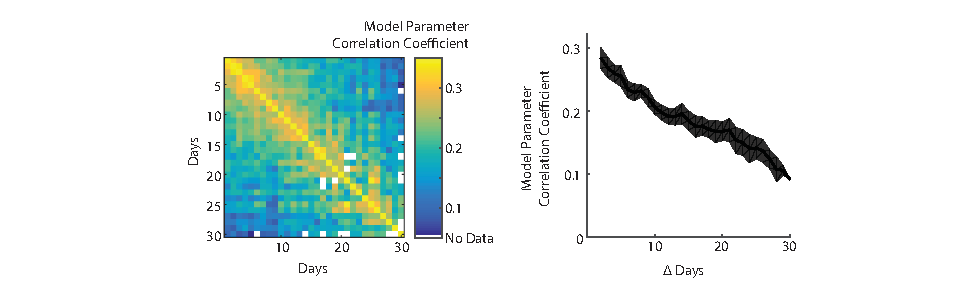
\includegraphics[width=\textwidth]{figures/4_glm_model_comparison.pdf}
\caption[Model comparison across days.]{\textbf{Model comparison across days.} Left: Kendall rank correlation coefficients of model beta coefficients fit on separate days. Diagonal values are 1. The values were averaged across all cells for each mouse and then averaged across mice. Each entry has a variable number of data points (and in some case no data points, white values) due to varying durations of imaging periods for mice and gaps between imaging sessions. See Figure \ref{fig:cell_selection} j for the number of mice at each interval. Right: Average correlation coefficient when fit and tested on data separated by n days. Shading indicates mean $\pm$ sem.  
\label{fig:model_comparison}}
\end{figure}

\bigskip

The changes in these activity-behavior relationships were made up of cells that lost well-modeled relationships, gained well-modeled relationships, and switched relationships across days. To quantify the prevalence of these events, we used a statistical threshold, based on shuffled data, to binarize model performance into models that predicted activity patterns above chance levels (significant predictions) and models that provided poor predictions of activity (Methods \ref{methods:analysis_of_model}). We then compared pairs of models fit on separate days for a given cell. If the models developed on one day provided good predictions of the activity patterns on the other day, then the cell was considered to have a consistent activity-behavior relationship (Figure \ref{fig:4_glm_across_population} a). Instead, if one model with a significant prediction of activity could be developed for one day's activity but not for the other day's activity, then the cell was considered to have lost or gained an activity-behavior relationship (Figure \ref{fig:4_glm_across_population} a). If models with significant predictions could be developed on both days but these models provided poor predictions of activity on the other day, then the cell was considered to have switched activity-behavior relationships (Figure \ref{fig:4_glm_across_population} a). The likelihood that a cell lacking an activity-behavior relationship gained such a relationship remained constant throughout the imaging period of weeks (26.8 $\pm$ 0.01$\%$ of cells) (Figure \ref{fig:4_glm_across_population} c). As the time interval between the compared days increased, the likelihood that a cell had a consistent relationship decreased, and the likelihood that a cell lost or switched a relationship increased (Figure \ref{fig:4_glm_across_population} c). After ~20 days, a cell that had a well-described activity-behavior relationship was more likely to have lost this relationship or switched to a different relationship than to have maintained its original relationship (Figure \ref{fig:4_glm_across_population} c). This rate of change was consistent throughout the entire imaging period. The likelihood that a cell gained, lost, switched or maintained an activity-behavior relationship from one day to the next remained constant throughout the imaging period of weeks. (Figure \ref{fig:4_glm_across_population} d)

\begin{figure}
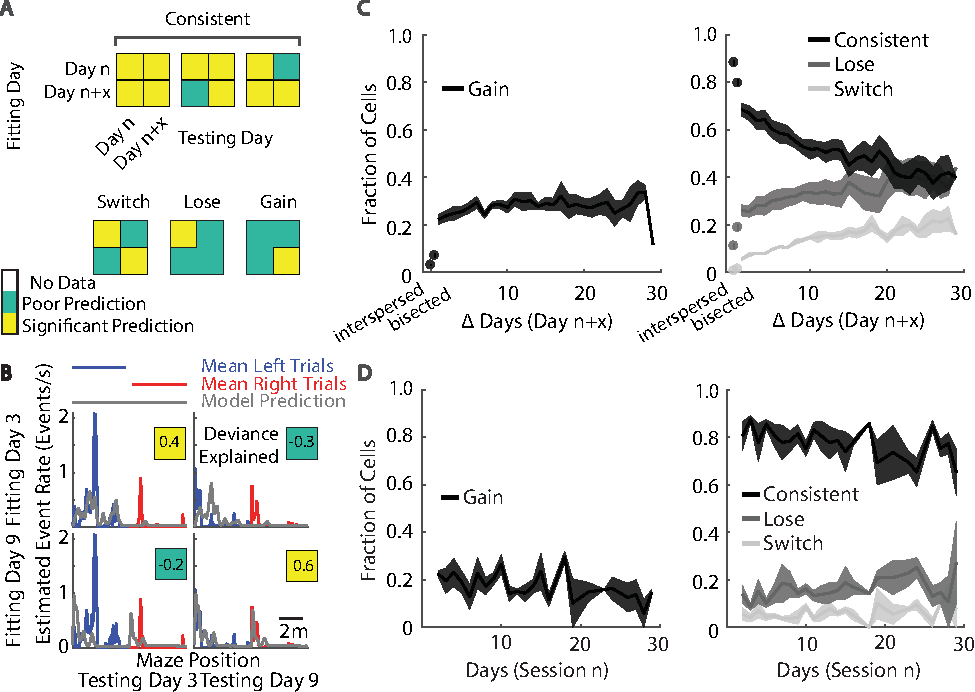
\includegraphics[width=\textwidth]{figures/4_glm_across_population.pdf}
\caption[Quantification of consistent, lost and gained activity-behavior relationships.]{\textbf{Quantification of consistent, lost and gained activity-behavior relationships. a,} Schematic for model comparisons binarized as significant and poor predictions using a statistical threshold of 0.2 deviance explained. This threshold was chosen based on fits from a bootstrap analysis in which behavior data were circularly shifted relative to neuronal activity (Methods \ref{methods:analysis_of_model}). Separate models were fit to an individual cell's activity on two days and tested on the fitted day or on the other day (as in Figure \ref{fig:glm_across} c). 
%
\textbf{b,} For an example cell, mean activity for white cue-left turn (blue) and black cue-right turn (red) trials on imaging days 3 and 9. One model was fitted on data from day 3 and another model was fitted on data from day 9. Each model was used to make a prediction (gray) about the neuron's activity based on behavioral data in a test set, either from the same day or the other day. The model fit quality was quantified as the deviance explained, which was thresholded and labelled as a 'poor prediction' or a 'significant prediction' (Methods \ref{methods:analysis_of_model}).
%
\textbf{c,} Left: For cells without a significant model prediction on day n, the fraction of cells that had a significant model prediction after a given interval. Right: For cells with a significant model prediction on day n, the fraction of cells with consistent (black), lost (medium gray), or switched (light gray) activity-behavior relationships after a given interval. Shaded area indicates mean $\pm$ sem (n = 5 mice; some large interval data points had fewer than 5 mice, see Figure \ref{fig:cell_selection}. Interspersed and bisected groups refer to models that were trained and tested on half of the data from a single session and compared to the corresponding model, trained and tested on the opposite half of the data from the same session. The interspersed group compares models that were built from interspersed chucks throughout the duration of the session and provides a baseline for change due to measurement noise. The bisected group compares models that were built from the first and second half of the session.
%
\textbf{d,} Left: For cells in which a model with a significant prediction of activity could not be developed on day n, the fraction of cells that had a model with a significant prediction of activity that could be developed on day n+1. Shaded region indicates mean $\pm$ sem across mice n = 5 (fewer mice on some later days).  Right: For cells with a significant model prediction on day n, the fraction of cells that had consistent (black), lost (medium gray), and switched (light gray) activity-behavior relationships on day n+1. Shaded region indicates mean $\pm$ sem. n = 5 (fewer mice on some later days). 
\label{fig:4_glm_across_population}}
\end{figure}

\bigskip

The rates at which neurons had changes in their activity-behavior relationships varied greatly across cells (Figure \ref{fig:glm_quant_stability} a). For each neuron, we calculated the likelihood that a model developed on one day provided a significant prediction of another day's activity (Figure \ref{fig:glm_quant_stability} b, left) and fit an exponential to this likelihood over time to define a metric of consistency for each cell (Figure \ref{fig:glm_quant_stability} b, right). Some neurons had slow decays and thus had relatively consistent activity-behavior relationships, whereas others had fast decays indicative of rapid changes. Over a 20 day interval, the large majority of neurons had a low likelihood of consistent models (Figure \ref{fig:glm_quant_stability} c). Only 7.3$\%$ of neurons had consistent activity-behavior relationships over the entire interval (defined as > 95$\%$ significant predictions after 10-20 days). To understand if the neurons with the most and least consistent activity-behavior relationships represented different types of behavioral information, we examined the contribution of various parameters to each cell's activity (the extent to which the behavioral parameter of interest modulated a given cell's model prediction, see Methods \ref{methods:contrib}). Cells with the most consistent and least consistent relationships had a distribution of contributions for trial type, position in the maze, running pattern, and inter-trial interval activity that overlapped with the distribution in the full population (Figure \ref{fig:glm_quant_stability} d). However, neurons with the least consistent relationships more often had greater contributions from trial type and maze position than neurons with the most consistent relationships (Figure \ref{fig:glm_quant_stability} d). Our results therefore suggest that there was a continuous distribution of stability in activity-behavior relationships across neurons, with activity related to learned task features (trial type and maze position) possibly having less consistency across time. 

\begin{figure}
\includegraphics[width=\textwidth]{figures/glm_quant_stability.pdf}
\caption[Distribution in the rate of change across cells in the population.]{\textbf{Distribution in the rate of change across cells in the population. a,} Mean activity for three example cells with varying consistency in activity-behavior relationships.  
%
\textbf{b,} Left: For example cells from panel \textbf{f}, matrix of fitting and testing comparisons as in panel . Right: Fraction of models with significant predictions as a function of time between the fitting and test days. Exponential fits are shown, weighted by the number of model comparisons that went into each data point. 
%
\textbf{c,} Histogram of the fraction of significant model predictions after 10-20 days of separation between the fitting and training days for all cells identified in at least 15 imaging days. n = 690 cells.

%
\textbf{d,} Contribution of different categories of behavior/task features to neuronal activity, estimated as the standard deviation of the linear part of the model (Methods \ref{methods:contrib}). For comparisons of cells with the 20 $\%$ most and 20 $\%$ least consistent models : Position/cue, p = 0.026; treadmill velocity, p = 0.98; whether the mouse was in the inter-trial interval, p = 0.79; t-test. Error bars indicate mean $\pm$ sem. n = 5 mice. Grey lines indicate 95 $\%$ confidence intervals for 20 $\%$ of randomly selected cells. 
%
\textbf{e,} On a given day, we identified for how many previous days the model of that day's activity provided a good prediction of previous day's activity. Models with significant predictions for data on $\ge$ 2 consecutive previous days were more likely to provide a good prediction in future days than models with significant predictions for data on only 1 previous day. $*$ indicates p < 0.05, t-test. 
\label{fig:glm_quant_stability}}
\end{figure}

\bigskip

The changes in activity-behavior relationships did not reflect independent relationships across days. Rather, consistent relationships in the recent past were predictive of consistent relationships in the short-term future. Neurons with a consistent activity-behavior relationship for two or more consecutive days prior to a particular imaging day were more likely to maintain that relationship than neurons which had a consistent relationship for only one of the immediately preceding imaging days (Figure \ref{fig:glm_quant_stability} e). These results suggest that neurons potentially operated with modes of activity that tended to persist for neighboring days such that a neuron's activity on each day was not independent of the recent history of its activity. However, the predictive power of recent consistency fell off after ten days, suggesting there was not a separate population of permanently consistent cells (Figure \ref{fig:glm_quant_stability} e).

\bigskip

The GLM analyses therefore suggest that the changes in activity we observed were likely due to unstable activity-behavior relationships, rather than changes in behavioral patterns across days. We further supported this finding by comparing the similarity of population activity patterns on trials with the most similar or least similar behavioral patterns across all days. The population activity was more similar on those trials with more similar behavioral features, measured as correlations between population activity vectors (Figure \ref{fig:behave_controls} a). However, the difference in activity similarity between the most and least similar behavioral trials was small compared to the population activity changes across time (Figure \ref{fig:behave_controls} a). In addition, we did not observe any evidence that the mouse forgot and re-learned the task on each day because mice performed at near perfect levels, even on the first few trials of each day (Figure \ref{fig:1_w_out_inact} b, Figure \ref{fig:behave_controls} b).

\begin{figure}
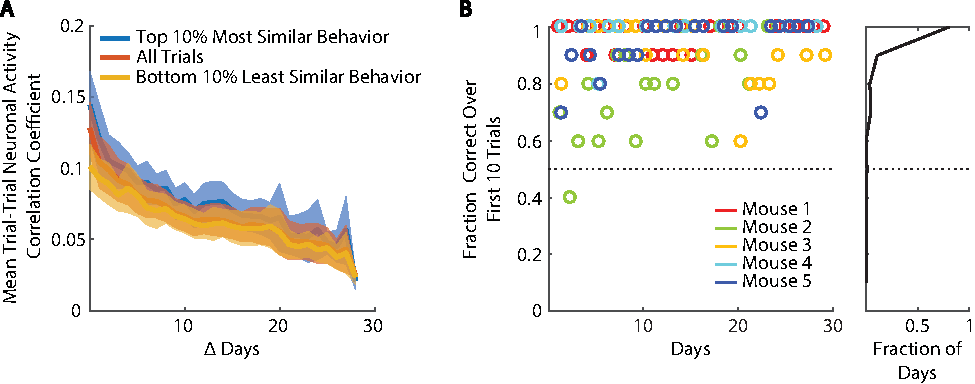
\includegraphics[width=\textwidth]{figures/behave_controls.pdf}
\caption[Behavioral change across days does not explain neuronal change.]{\textbf{Behavioral change across days does not explain neuronal change. a,} Similarity in population activity as a function of days separating sessions for the trials with the most or least similar behavioral patterns. Behavioral patterns were compared using a mean vector of all measured behavioral parameters (forward speed, clockwise speed, view angle, position along stem axis, and position along arm axis) at each position in the maze (5 parameters x 21 spatial bins). Similarity was determined as the pairwise trial-trial correlation coefficient of this behavioral parameter vector. Population activity patterns were compared using a vector of population activity (neurons x 21 spatial bins). Similarity was determined as the pairwise trial-trial correlation coefficient of this population activity vector. Trials with more similar behavioral patterns were often found on sessions that were separated by a smaller time interval. However, there were some pairs of sessions in the top 10 $\%$ most similar that spanned the full duration of our experiment, and some pairs of sessions in the 10 $\%$ least similar that were found in neighboring days. 
%
\textbf{b,} Left: Behavioral performance over the first ten trials on each imaging day for all mice. Right: Cumulative density plot of behavioral performance on the first ten trials of imaging days. 
\label{fig:behave_controls}}
\end{figure}

\subsection{Consistent statistical features of population activity on each day} \label{sec:chap3_set_point}

Despite these changes in the activity of individual neurons, we noticed that consistent patterns were present in the population activity on each day. As shown above, neuronal activity that tiled the full trial duration was present on each day and was made up of different neurons across days (Figure \ref{fig:2_all}). The distribution of population activity across the trial was not uniform, but this distribution was highly similar across all days in a given population of neurons (Figure \ref{fig:5_set_point} a-b). In addition, on each day, a decoder for trial type based on population activity achieved similar levels of performance and had similar distributions of performance across time points in the trial (Figure \ref{fig:5_set_point} c-d). Interestingly, in each population of neurons from different mice, differences between mice were maintained across days. For example, the population of neurons in one mouse (red) had higher decoding accuracy of trial type than did the population of neurons in another mouse (green) across all days (Figure \ref{fig:5_set_point} d). These differences were maintained with a similar shape across the duration of the trial (Figure \ref{fig:5_set_point} c). Many other properties of population activity had similar distributions on each day, including for neuron-neuron activity correlations (Figure \ref{fig:5_set_point} e-f, trial-trial population activity correlations (Figure \ref{fig:5_set_point} g-h), estimated population firing rates (Figure \ref{fig:5_set_point} i-j), and decoding accuracy of trial type for individual neurons (Figure \ref{fig:5_set_point} k-l). These results indicate that even though properties of activity in individual neurons changed across time, the statistical features of population activity were largely consistent over weeks. Therefore, the population appeared to have a 'set point' of similar activity each day, using different neurons, and neurons in different ways, to achieve this steady state.

\begin{figure}
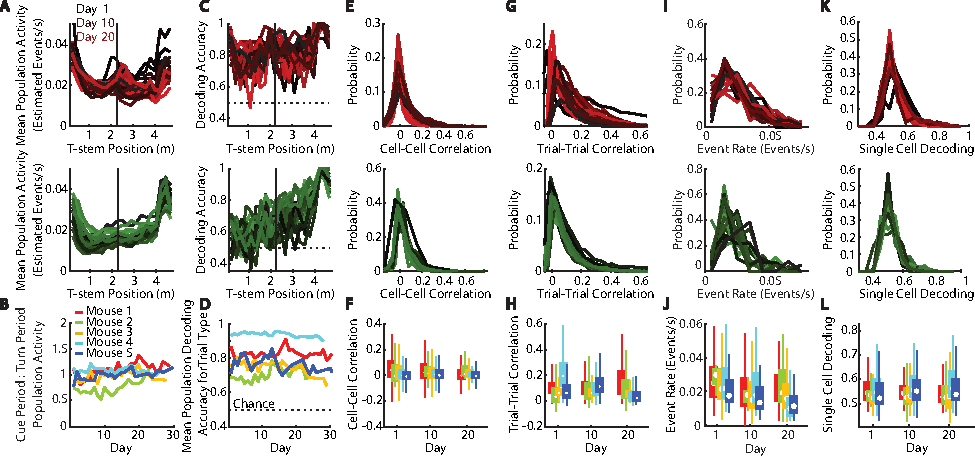
\includegraphics[width=\textwidth]{figures/5_set_point.pdf}
\caption[Stable statistical features of population activity.]{\textbf{Stable statistical features of population activity. a,} For two example mice, the mean population activity as a function of position in the maze. Darker to lighter colors indicate earlier to later days.
%
\textbf{b,} Ratio of activity in the cue period to the delay period on each day for each mouse.
%
\textbf{c,} For two example mice, population decoding accuracy of trial type as a function of position in the maze. Separate decoders were trained at each spatial bin and on each day. 
%
\textbf{d,} Population decoding accuracy of trial type for each mouse on each day. 
%
\textbf{e,} For two example mice, distributions of cell-cell correlations of deconvolved calcium signals smoothed with a 2-second sliding window across all pairs of neurons on each day. 
%
\textbf{f,} Summary of cell-cell correlation distributions for all mice for days 1, 10 and 20. Boxes represent the 25th and 75th percentiles, white dots indicate the mean, and whiskers show the 99 $\%$ range of the data.
%
\textbf{g-l,} Same as in panels \textbf{e-f}, except for correlations of the matrix of population activity (cells x maze position) between trials of the same type \textbf{g-h}, activity event rates in the population of neurons estimated from deconvolved calcium signals \textbf{i-j}, and classification accuracy of trial type based on single-cell activity patterns \textbf{k-l}.

\label{fig:5_set_point}}
\end{figure}

\subsection{Decoding of information from dynamic neuronal representations} \label{sec:chap3_peaks}

The changes in neuronal activity-behavior relationships over time raise questions about how information could be read out from such a dynamic neuronal population over days and weeks. One possibility is that the cells with the most consistent activity-behavior relationships are those that preferentially carry information for the readout. Alternatively, it could be possible that the activity in the cells with less consistent activity-behavior relationships also allows decoding of information over time. We investigated this issue by testing various decoding strategies for reading out the trial type on the basis of population activity.

\bigskip

We first trained and tested a linear decoder on each day separately using all neurons (as in Figure \ref{fig:5_set_point} c-d). We found trial type information could be decoded throughout the duration of the trial, with higher decoding accuracies at the end of the trial, when the mouse executed a turn at the T-intersection (Figure \ref{fig:decoding} a). We then compared the decoding performance using the cells with the most consistent activity-behavior relationships and the least consistent relationships, defined by exponential fits of model performance decay over time (from Figure \ref{fig:glm_across} b, see Methods \ref{methods:analysis_of_model}). The population of cells with the least consistent activity-behavior relationships had better decoding accuracy throughout the majority of the trial than did the cells with the most consistent relationships. In the final segment of the trial, when the mouse executed a turn, decoding accuracies were similar between groups (Figure \ref{fig:decoding} b). 

\begin{figure}
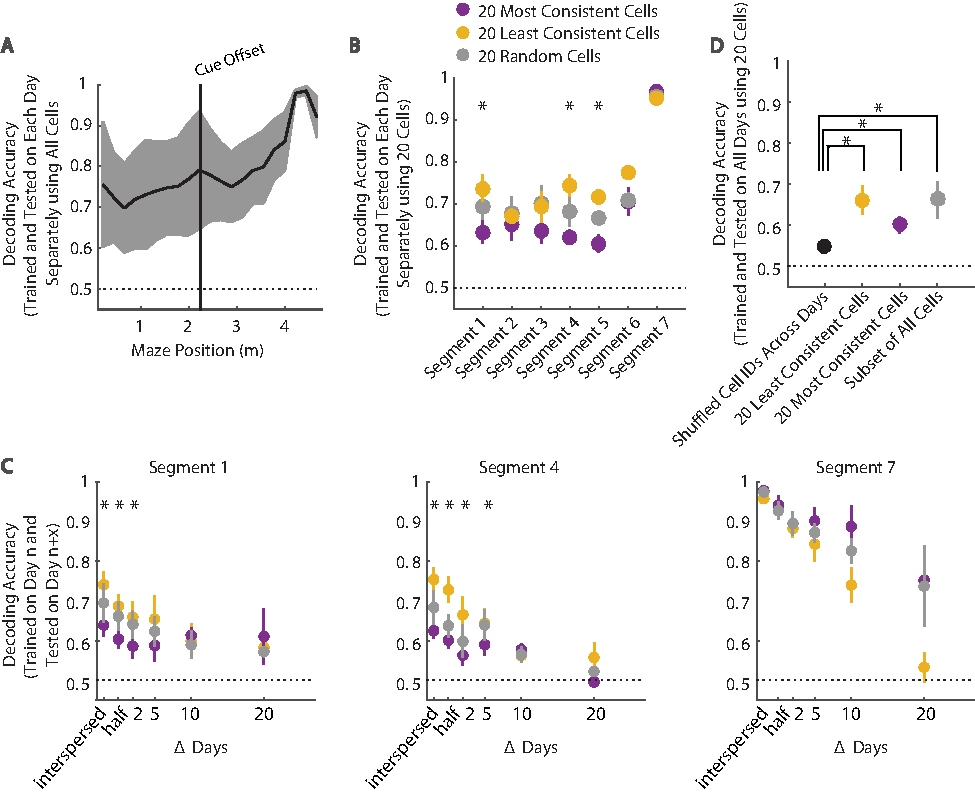
\includegraphics[width=\textwidth]{figures/6_decoding_unstable_stable_7bins_small.pdf}
\caption[Decoding task information across days.]{\textbf{Decoding task information across days. a,} Population decoding accuracy of trial type on correct trials as a function of position in the maze. The decoder was trained and tested on the same day. Separate classifiers were trained at each spatial bin and on each day. Shaded region indicates mean $\pm$ sem. n = 5 mice.
%
\textbf{b,} Population decoding accuracy of trial type on correct trials using 20 cells with the least consistent activity-behavior relationships (yellow), 20 cells with the most consistent activity-behavior relationships (purple), and 20 randomly selected cells (gray) for 7 segments of the trial, which included 3 spatial bins each. The decoder was trained and tested on the same day. Error bars indicate mean $\pm$ sem. n = 5 mice. $*$ indicates p < 0.05, t-test, between least consistent and most consistent groups. 
%
\textbf{c,} Decoding performance when the decoder was trained on a given session and tested on a later session for segment one (left) segment four (middle) and segment seven (right). Error bars indicate mean $\pm$ sem. n = 5,5,4,4,2 mice for $\Delta$ days 0,2,5,10,20 respectively. $*$ indicates p < 0.05, t-test, between least consistent and most consistent groups. Interspersed and bisected groups refer to population decoders trained on odd/even trials and tested on even/odd trials or trained on the first/second half and tested on the second/first half of a single session respectively. 
%
\textbf{d,} Decoding performance when the decoder was trained on data from all days and tested on a separate set of data from all days. In addition to the conditions from panel \textbf{b} and \textbf{c}, decoding was performed with cell IDs shuffled separately for each individual day (cells did not have a consistent ID across days). Error bars indicate mean $\pm$ sem. n = 5,5,4,4,2 mice for $\Delta$ days 0,2,5,10,20 respectively.  $*$ indicates p < 0.05, t-test, between shuffled cell IDs and the indicated other group.
\label{fig:decoding}}
\end{figure}

\bigskip

To analyze the stability of information in activity patterns, we tested decoding performance across days. We trained a decoder on a given day and tested it on subsequent days (Figure \ref{fig:decoding} c). When considering a random subset of cells, decoding performance decreased as the interval between compared days increased. This result was present throughout the duration of the trial (Figure \ref{fig:decoding} c). In the cells with the most consistent activity-behavior relationships, decoding performance was low and consistent across time for the majority of the trial (Figure \ref{fig:decoding} c, left and middle). For the final segment of the trial, the decoding performance in these cells was high and consistent over days (Figure \ref{fig:decoding} c, right). As expected, the performance of a decoder trained on one day and tested on other days decreased as a function of time for the cells with the least consistent activity-behavior relationships (Figure \ref{fig:decoding} c). Interestingly, however, over intervals within one week, these cells performed better in the majority of the trial than the cells with the most consistent relationships (Figure \ref{fig:decoding} c, left and middle). Together, these results indicate that the information in the population was not stable over time, but some information remained in the population for days and weeks, even in neurons with the least consistent activity patterns.

\bigskip

If the relevant information for the task must be read out near the time the mouse executes a turn, then it might be beneficial to weight strongly the activity of the cells with the most consistent activity-behavior relationships. In contrast, if information in the T-stem is more relevant for behavior, then weighting the activity of the cells with the less consistent relationships might be beneficial. Our cue and delay period inactivation experiments demonstrate that PPC is required during the cue period only, when the least consistent cells had more information about trial type. Therefore, it is possible that the task-relevant information in the cells with the least consistent activity-behavior relationships could be of importance for PPC's role in this task.

\bigskip

These results suggest that to maintain high levels of information across time, an ideal readout would need to change in a coordinated manner with the encoding network. However, we wanted to test if it might be possible to identify a stable readout in the form of a single decision plane that could be used across all days to separate trials of different types on every day. We combined all imaging days together and trained a decoder on a subset of trials and tested this single decision boundary on other trials that were distributed across all days. We compared the performance of this combined-day decoder using only the neurons with the least consistent activity-behavior relationships, the most consistent relationships, or a random sample of all neurons (Figure \ref{fig:decoding} d). In these cases, the cells with the least consistent relationships provided information at a similar level as the other groups and allowed decoding of trial type above chance levels. When the identities of the cells were shuffled independently on each day, the ability to find a stable readout decreased significantly, indicating that the decoding performance required the structure of the population activity over days (Figure \ref{fig:decoding} d). This analysis therefore reveals that, for the binary classification of trial type over the time intervals examined, it is possible to find a stable readout of population activity that performs above chance levels, even from the most dynamic population of neurons. However, to achieve higher performance, a readout that changes dynamically with the encoding network would likely be necessary. 

\section{Discussion}
Our results reveal that during stable performance of a learned navigation task, the activity patterns in PPC were variable over the timescales of days and weeks. These findings indicate that through the course of learning, neuronal activity patterns in PPC did not converge to a single representation. Rather, there appeared to be a set of activity patterns in the PPC population that were similarly sufficient for the task. Importantly, many statistical features of the population activity were consistent across days, such that the population appeared to reach a set point. However, the PPC neurons that were used in this representation, and how these PPC neurons were used, changed across days.

\section{Acknowledgements}
We thank Ofer Mazor and members of the Harvey lab for comments on the manuscript. We thank Paola Patella and Matthias Minderer for contributing to the design and setup of the inactivation experiments. We also thank the Research Instrumentation Core at Harvard Medical School. This work was supported by a Burroughs-Wellcome Fund Career Award at the Scientific Interface, the Searle Scholars Program, the New York Stem Cell Foundation, the Alfred P. Sloan Research Foundation, a NARSAD Brain and Behavior Research Young Investigator Award, NIH grants from the NIMH BRAINS program (R01MH107620) and NINDS (R01NS089521), an Armenise-Harvard Foundation Junior Faculty Grant, a Edward R. and Anne G. Lefler Center Predoctoral Fellowship and Junior Faculty Award, the Albert J. Ryan Fellowship, and the Stuart H.Q. and Victoria Quan Fellowship. C.D.H. is a New York Stem Cell Foundation Robertson Neuroscience Investigator. 

\section{Author contributions}
L.N.D and C.D.H. conceived of the project. N.L.P. designed and performed inactivation experiments and analyzed associated data. M.M. designed retinotopy experiments and analyses and built the widefield microscope. S.N.C. and M.M. designed cell selection algorithm and gui for extracting single session ROI maps. L.N.D. designed across session alignment algorithm and gui for aligning ROI maps across days. L.N.D and C.D.H designed all other experiments and analyses, and L.N.D. performed these experiments and analyses. L.N.D. and C.D.H. wrote the manuscript. 

\section{Data analysis methods}
\subsection{General analysis procedures}
For visualization of mean and single trial activity, activity was spatially binned into 66 segments (60 in the stem and 6 in the arms) followed by ~2 seconds (10 imaging frames) during the inter-trial interval. Spatially binned segments typically contained 1 imaging frame each per trial. Data was interpolated to fill in gaps in which a bin contained no imaging frames on a trial. These analyses were only used for fine-resolution measurements of locations of peak activity. For the majority of the analyses (all except Figure \ref{fig:2_all}), we binned the data into larger segments (21 segments, 23 cm/bin). Neuronal activity and behavioral parameters were averaged in each bin in this case. Each bin typically contained 2-3 frames/trial. Unless otherwise noted, all analyses were performed on correct trials only. Correlation coefficients were calculated from Pearson's correlations unless otherwise noted.

\subsection{Identification of significant peaks of activity}\label{methods:peaks}
Here we used 60 spatial bins during the T-stem rather than 21 spatial bins because we were interested in achieving greater resolution of spatial reorganization. Mean activity across 60 spatial bins were calculated for correct white cue-left turn and black cue-right turn trials. To identify statistically significant peaks of activity, behavior data time courses were circle-shifted by a random amount relative to neuronal activity time courses, and new means were calculated for 1000 random shifts. All locations where the mean activity in the unshifted data was greater than activity in 950 shuffles for three consecutive bins were considered to contain a significant peak of activity. For all analyses where peaks were compared across days, we tracked peaks that were labelled with high confidence (unshifted data was greater than activity in 990 shuffles for three consecutive bins). Peaks were labelled as 'gained' or 'lost' if in the absent session, there was below 95 $\%$  significance for a peak at that location. We found this gap between thresholds for the presence or absence of a peak to be important for limiting measurement noise. By these criteria for change, we found peak consistency across odd and even trials within one session to be 83.2 $\pm$ 2.1  $\%$ .

\subsection{Encoding model}
On each day separately, we fit a Poisson Generalized Linear Model \citep{Friedman2010} to the estimated event rates of each cell based on measured behavioral and task variables. While our estimated event rates were not necessarily Poisson distributed, mean responses scaled with the variance and rates were larger than zero, suggesting that the Poisson model was appropriate for our data.

\subsubsection{Model parameters}\label{methods:model_param}
All measured behavioral and task-related variables were temporally averaged into bins to match the sampling rate of imaging frames. Variables include x and y position in the virtual world, running speed on the pitch and roll axes of the spherical treadmill, visual cue onset and offset locations, reward delivery events and trial end (Figure \ref{fig:4_filters}). Variables provided input for basis functions that were distributed either in space or in time to produce 144 predictors in total. The maze was divided into 36 spatial boxcar filters and convolved with a Gaussian filter separately for right and left turn trials to make the first 72 filters. The onset of each visual cue contributed 4 basis functions (16 in total for all four cues) that spanned the first 2 seconds of the trial. For cue offset (delay period onset), 2 basis functions extended for 1 second preceding cue offset, and 4 basis functions extended for 2 seconds following cue offset (24 in total for all four cues). Running speed signals were extended 1 second forward and backward in time for translational, clockwise and counterclockwise rotational motion (4 filters forward and 4 filters backward for each of 3 speed signals for a total of 24 filters) to model predictive and responsive signals. Trial-end and reward events each contributed 4 basis functions that extended for 2 seconds forward in time (8 filters total). All temporal filters spanned 1 second, overlapping and evenly distributed within each set.

\subsubsection{Fitting}\label{methods:fitting}
We used the glmnet package in R to fit GLMs. Each day was divided into 10 evenly distributed chunks (first tenth of session, second tenth of session, and so on) and then sub-divided into 11 numbered pieces within each chunk. All pieces with the same number were then combined into groups 1-11. This resulted in 11 groups that contained data that was evenly distributed across the imaging session (Figure \ref{fig:4_glm_tutorial}). Seven of these groups were randomly chosen and used as cross validation folds during fitting, and the other three groups were combined and used to test model predictions (7 groups made up 73 $\%$  fitting and 3 groups made up 27 $\%$  testing predictions). For some figures, we compare models that were trained on a subset of data from a single session. First we divided data from a single session into halves, either interspersed chunks throughout the duration of the session (interspersed) or simply the first and second half of the session (bisected). We then treated these halves as independent sessions that were divided as we previously describe (73 $\%$  fitting and 27 $\%$  testing predictions). These models were only used for comparison to the appropriate opposite half within a single session. Parameters were fitted for each cell separately with elastic net regularization consisting of 10 $\%$  L2 and 90 $\%$  L1 methods. Model fitting was conducted on the Orchestra High Performance Compute Cluster at Harvard Medical School. This shared facility is partially supported by NIH through grant NCRR 1S10RR028832-01.
 
\subsubsection{Analysis of model}\label{methods:analysis_of_model}
Deviance explained was used as the metric of model fit. It was calculated by comparing the activity predicted by the model to the actual activity, based on the average real and predicted activity levels on white cue-left and black cue-right turn trials. Deviance explained was calculated based only on data not included in the fitting procedure. It was compared to a null model in which the predicted event rate was 1 (the normalized mean rate of the entire fitting set). We also computed deviance explained using predictions of the full time series of activity for single frames. In this case, the distribution of fits was similar, except lower than for trial-averaged data, as expected. To determine whether a model prediction described test data significantly above chance, we compared the deviance explained to the distribution of deviance explained for models in which, before model fitting, the time series of neuronal activity was circle-shifted relative to the time series of behavior data. We found the upper limit of deviance explained in models that were fit on shuffled data to be 0.2 (for trial-averaged activity). Therefore, we determined models with greater than 0.2 deviance explained on test data to have predictions significantly above chance performance. Cells with activity that could not be significantly predicted by our models could still have behaviorally relevant activity patterns that were simply not described by our set of filters. Therefore, when we refer to cells having gained or lost activity-behavior relationships, we refer specifically to the set of relationships included in our models. 
\bigskip
By comparing model fits between any two days or between subsets of data from a single day, we could determine whether a given neuron's activity-behavior relationship was consistent over time, gained or lost a relationship to a behavioral feature, or switched from encoding a particular set of behavioral features to encoding another. If models with significant predictions could be fit on each individual day's data for a given pair of days and if the models also provided significant predictions of the other day's activity, then we called the activity-behavior relationship consistent. If models with significant fits could be fit on each individual day's data for a given pair of days and if the models did not provide significant predictions on the other day, we determined a switch in activity-behavior relationship had occurred. If only one day had a model that could predict the neuron's activity significantly well, then we concluded that a gain or a loss of activity-behavior relationship had occurred. This approach works well when behavioral variables are not highly correlated. However, if behavioral variables are very highly correlated, then it is difficult for the model to determine to which variable weight should be attributed. If variables were highly correlated on one day but not correlated in another day, then incorrect assignments of switches in activity-behavior relationships could emerge. To be conservative and to account for any potential cases in which non-modeled variables were highly correlated with modeled variables (on some days but not others), we did not require symmetry in model performance across days for an activity-behavior relationship to be considered consistent. That is, if a model prediction on day i and day j both had significant predictions of activity and if the model from day i predicted well the activity from day j, but not vice versa, then a consistent activity-behavior relationship would still be considered to be present. In this case, if behavior variables x and y were highly correlated on day j but not on day i, then the model on day j might incorrectly attribute weights on day j leading to a poor prediction on day i. However, because the variables x and y were not highly correlated on day i, then the model would correctly attribute weights on day i, successfully predicting activity on day j despite having correlated variables x and y on day j. This method would still fail to identify a consistent activity-behavior relationship if the 'real' encoded feature (for example, mental state) was correlated with different filters in the model on each day. These subtle behavioral confounds are difficult to remove completely and should be considered in the interpretation of this work and most other behavioral studies. Through the use of virtual reality we could control the sensory environment and track behavioral metrics with great precision, incorporating these features into our models and thus minimizing the aforementioned concerns.

\subsubsection{Metric of consistency in activity-behavior relationships}\label{methods:metric_consistency}
We defined the consistency of activity-behavior relationships for each cell by the likelihood that an encoding model fit on a given day continued to provide significant predictions of the cell's activity for days and weeks. We found the fraction of models that provided a significant prediction of a given cell's activity over each interval between fitting and prediction sets (1-30 days). We then fit an exponential decay, weighting each point by the number of model comparisons available (for example, there were more model comparisons where $\Delta$ days = 1 than $\Delta$ days = 30). We only included cells that had significant fits on at least half of days where $\Delta$ days = 0 because cells with a low starting point necessarily had slow decays (the fraction of significant model fits was bounded between the y-intercept and zero).

\subsubsection{Contribution of task and behavioral features to the activity of a cell}\label{methods:contrib}
To calculate the contribution of each task and behavioral variable to a given model, we computed the standard deviation of the linear part of the model that was related to the behavioral variable of interest (the standard deviation of beta coefficients crossed with relevant behavioral filters of behavioral data). This provided us with the extent to which a behavioral variable modulated the activity of the neuron. For filter groupings in position/cue, velocity and ITI contribution calculation see Figure \ref{fig:4_filters}.


\subsection{Decoding}\label{methods:decoding}
We used C-Support Vector Classification with a linear kernel for all decoders. For some decoders, we considered the activity of single cells (Figure \ref{fig:3_all} and \ref{fig:5_set_point} k). In these cases, the decoder was trained using data from all 21 spatial bins in the trial. In other cases, in which we wanted to assess the time course of information, we trained decoders on each spatial bin separately using the activity of all neurons or subsets of neurons (Figure \ref{fig:5_set_point} a and \ref{fig:decoding}). When decoders incorporated a smaller number of cells (20 cells each for subgroups in Figure \ref{fig:decoding}) we divided the maze into larger bins to account for the fact that each only had trial type information for a small portion of the trial. For decoding analyses, the data were divided into two-thirds for training/validation and one-third for testing. The regularization weight hyperparameter C was selected using a random search with 10-fold cross validation on a subset of training sets across mice. The specific setting of the hyperparameter did not greatly affect the accuracy of our decoders. The same hyperparameter value (C = 100) was used for all data sets. Significant decoding accuracies in Figure \ref{fig:3_all} were determined by bootstrap analysis in which behavioral data were circularly rotated relative to each cell's neuronal activity. Cells in which real data performed better than 950 of 1000 shuffles were determined to have significant decoding accuracy. Using this statistical threshold, it is thus expected that 5 $\%$  of cells would have significant decoding accuracy by chance.